\documentclass[a4paper, 11pt]{article}
\usepackage{geometry}
\geometry{letterpaper, margin=1in}
\usepackage{graphicx}
\graphicspath{ {images/} }

\usepackage{amsmath}
\usepackage{amssymb}  
\usepackage{amsthm}
\usepackage{ulem}

\usepackage{enumitem}


\usepackage{pdfpages} % for including full pdf pages

\usepackage{empheq}

\usepackage{listings}


%format to allow bolded theorems, corollaries, etc...
\newtheorem*{theorem}{Theorem}
\newtheorem*{corollary}{Corollary}
\newtheorem*{lemma}{Lemma}
\newtheorem*{definition}{Definition}
\newtheorem*{Example}{Example} 
\newtheorem*{Remark}{Remark}

% stop typing \mathbb a thousand times 
\newcommand{\R}{\mathbb{R}}
\newcommand{\C}{\mathbb{C}}
\newcommand{\F}{\mathbb{F}}
\newcommand{\E}{\mathbb{E}}
\newcommand{\sphere}{\mathbb{S}}

% commands for bra-ket notation
\newcommand{\bra}[1]{\ensuremath{\left\langle#1\right|}}
\newcommand{\ket}[1]{\ensuremath{\left|#1\right\rangle}}
\newcommand{\bracket}[2]{\ensuremath{\left\langle #1 \middle| #2 \right\rangle}}
\newcommand{\matrixel}[3]{\ensuremath{\left\langle #1 \middle| #2 \middle| #3 \right\rangle}}
\newcommand{\expectation}[1]{\ensuremath{\left\langle #1 \right\rangle}}

% vector stuff
\newcommand{\basis}[1]{\hat{\mathbf{e}}_#1}
\newcommand{\unit}[1]{\hat{\boldsymbol{#1}}}
\newcommand{\bvec}[1]{\vec{\boldsymbol{#1}}}


% change margins for solution
\newenvironment{solution}{%
	\begin{list}{}{%
			\setlength{\topsep}{0pt}%
			\setlength{\leftmargin}{0.5cm}%
			\setlength{\rightmargin}{0.5cm}%
			\setlength{\listparindent}{\parindent}%
			\setlength{\itemindent}{\parindent}%
			\setlength{\parsep}{\parskip}%
		}%
		\item[]}{\end{list}}



\begin{document}
\noindent
\large\textbf{Assignment 4: Design} \hfill \textbf{John Waczak} \\
\normalsize CS 162 \hfill  Date: \today 
\par\noindent\rule{\textwidth}{0.4pt} \\\\



\section*{Understanding the problem}

\textit{In your own words, explain what YOU think the problem is asking you to
  do.  Document your uncertainties about the problem and anything else that you
  feel was unclear or vague}\\

The problem asks us to design a game in which a player is within a cave system
and seeks to find a chest of gold. The player may move between rooms in which a
variety of events can occur. The player may fall into a bottomless pit, be
transported by a super bat, find the golden treasure, or wake up the Wumpus. If
the player enters the room with the Wumpus,  it awakens and proceeds to eat her.
Before moving though, the player may choose to fire an arrow (of which she has
3). If the arrow reaches the Wumpus (within a distance of 3 rooms), it dies.
Otherwise, the arrow is wasted. Once the player has found the treasure, they
must return to the initial room to escape up the escape rope. 
\section*{Devising a plane/design}

\textit{Provide an algorithm/pseudo code to help solve the problem. In addition,
  draw pictures/flow charts to help you devise your plan, as well as any other
  design decisions you make, such as how to manage your time, how to decompose
  the problem, where to start first, etc. }\\ 

I will implement a polymorphic class structure. The event class will be abstract
from which the wumpus, super bat, bottomless pit, and golden treasure classes
are derived. I will use a ``rooms'' class to manage a dynamic array of events.
With this structure, the flow of the program will be implemented as shown in the
following flow chart.

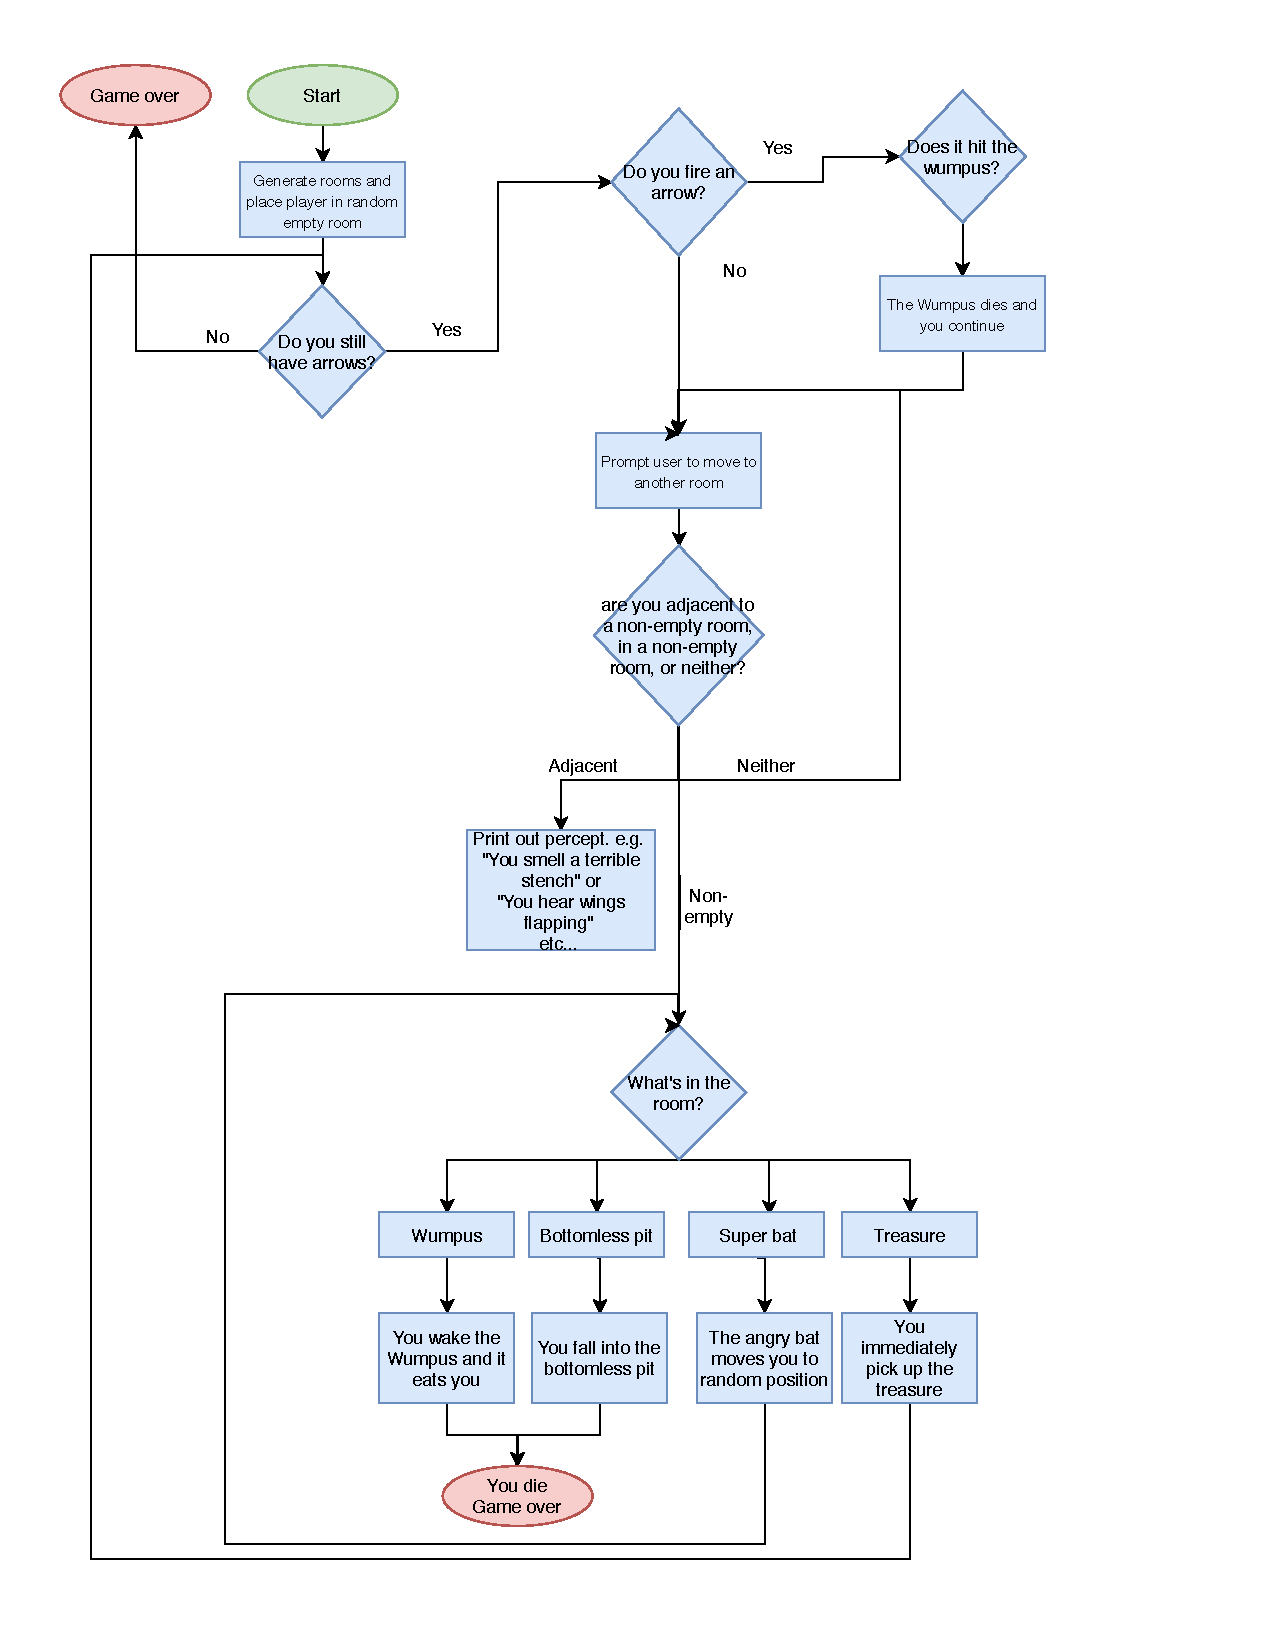
\includepdf{images/hw4_flow.pdf}

\section*{Looking back / testing}

\textit{This includes any checking/self-reflection you did while solving the
  problem, which includes using a calculator to make sure the output is correct,
  testing to make sure your code executes correctly and behaves the way you
  expect under specific circumstances, using sources of information to make
  sense of the results, etc. However, you need to think about the input prior to
  implementation!!!}\\
\vspace{5em}

\begin{center}
 \begin{tabular}{l|l} % <-- Alignments: 1st column left, 2nd middle and 3rd right, with vertical lines in between
   \textbf{Input} & \textbf{Expected} \\
    &    \\
   \hline
   player moves near room with event & percept is printed to the screen \\
   player fires arrow in empty direction& ``nothing interesting happens...'' is printed\\
   player fires arrow at wumpus  & ``you hear a loud YAAAAARRGH! followed by silence'' is printed\\
   player runs out of arrow & ``Game over'' is printed \\
   Debug mode engaged & detailed map is printed to screen \\
   you walk into bottemless pit & ``You fall to your death. Game over!'' is printed \\
   you walk into super bat & you are moved to random room 
 \end{tabular}
\end{center}

\end{document}
